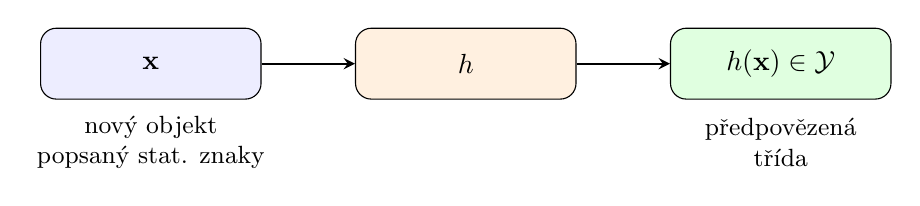
\begin{tikzpicture}[
    >=stealth,
    box/.style={
        draw,
        rounded corners=2mm,
        minimum width=28mm,
        minimum height=9mm,
        align=center,
        fill=blue!7
    },
    arr/.style={->, thick}
]
    \node[box] (x) at (0,0) {$\mathbf{x}$};
    \node[box, fill=orange!12] (h) at (4,0) {$h$};
    \node[box, fill=green!12] (y) at (8,0)
        {$h(\mathbf{x})\in\mathcal{Y}$};

    \draw[arr] (x) -- (h);
    \draw[arr] (h) -- (y);

    \node[font=\small, align=center] at (0,-1)
        {nový objekt\\popsaný stat. znaky};
    \node[font=\small, align=center] at (8,-1)
        {předpovězená\\třída};
\end{tikzpicture}
